\printconcepts

\exercise{The dot product of two vectors is a \underline{\hskip .5in}, not a vector.}{Scalar}

\exercise{How are the concepts of the dot product and vector magnitude related?}{The magnitude of a vectors is the square root of the dot product of a vector with itself; that is, $\norm{\vec v} = \sqrt{\vec v\cdot \vec v}$.}

\exercise{How can one quickly tell if the angle between two vectors is acute or obtuse?}{By considering the sign of the dot product of the two vectors. If the dot product is positive, the angle is acute; if the dot product is negative, the angle is obtuse.}

\exercise{Give a synonym for ``orthogonal.''}{``Perpendicular'' is one answer.}

\printproblems

\exerciseset{In Exercises}{, find the dot product of the given vectors.
}{

\exercise{$\vec u = \la 2,-4\ra$, $\vec v = \la 3,7\ra$
}{$-22$
}

\exercise{$\vec u = \la 5,3\ra$, $\vec v = \la 6,1\ra$
}{$33$
}

\exercise{$\vec u = \la 1,-1,2\ra$, $\vec v = \la 2,5,3\ra$
}{$3$
}

\exercise{$\vec u = \la 3,5,-1\ra$, $\vec v = \la 4,-1,7\ra$
}{$0$
}

\exercise{$\vec u = \la 1,1\ra$, $\vec v = \la 1,2,3\ra$
}{not defined
}

\exercise{$\vec u = \la 1,2,3\ra$, $\vec v = \la 0,0,0\ra$
}{$0$
}
}

\exercise{Create your own vectors $\vec u$, $\vec v$ and $\vec w$ in $\mathbb{R}^2$ and show that $\vec u\cdot (\vec v+\vec w) = \vec u\cdot \vec v + \vec u\cdot \vec w$.}{Answers will vary.}

\exercise{Create your own vectors $\vec u$ and $\vec v$  in $\mathbb{R}^3$  and scalar $c$ and show that $c(\vec u\cdot \vec v) = \vec u\cdot (c\vec v)$.}{Answers will vary.}

\exerciseset{In Exercises}{, find the measure of the angle between the two vectors in both radians and degrees.}{

\exercise{$\vec u =\bracket{1,1}$, $\vec v =\bracket{1,2}$}{$\theta = 0.3218 \approx 18.43^\circ$}

\exercise{$\vec u =\bracket{-2,1}$, $\vec v =\bracket{3,5}$}{$\theta = 1.6476 \approx 94.4^\circ$}

\exercise{$\vec u =\bracket{8,1,-4}$, $\vec v =\bracket{2,2,0}$}{$\theta = \pi/4 = 45^\circ$}

\exercise{$\vec u =\bracket{1,7,2}$, $\vec v =\bracket{4,-2,5}$}{$\theta = \pi/2 = 90^\circ$}

}


\exerciseset{In Exercises}{, a vector $\vec v$ is given. Give two vectors that are orthogonal to $\vec v$.
}{

\exercise{$\vec v = \la 4,7\ra$
}{Answers will vary; two possible answers are $\la -7,4\ra$ and $\la 14,-8\ra$.
}

\exercise{$\vec v = \la -3,5\ra$
}{Answers will vary; two possible answers are $\la 5,3\ra$ and $\la -15,-9\ra$.
}

\exercise{$\vec v = \la 1,1,1\ra$
}{Answers will vary; two possible answers are $\la 1,0,-1\ra$ and $\la 4,5,-9\ra$.
}

\exercise{$\vec v = \la 1,-2,3\ra$
}{Answers will vary; two possible answers are $\la 2,1,0\ra$ and $\la 1,1,1/3\ra$.
}
}

\exerciseset{In Exercises}{, vectors $\vec u$ and $\vec v$ are given. Find $\proj uv$, the orthogonal projection of $\vec u$ onto $\vec v$, and sketch all three vectors on the same axes.
}{

\exercise{$\vec u = \la 1,2\ra$, $\vec v = \la -1,3\ra$\label{ex:10_03_ex_21}
}{$\proj uv = \la -1/2,3/2\ra$.
}

\exercise{$\vec u = \la 5,5\ra$, $\vec v = \la 1,3\ra$
}{$\proj uv = \la 2,6\ra$.
}

\exercise{$\vec u = \la -3,2\ra$, $\vec v = \la 1,1\ra$
}{$\proj uv = \la -1/2,-1/2\ra$.
}

\exercise{$\vec u = \la -3,2\ra$, $\vec v = \la 2,3\ra$
}{$\proj uv = \la 0,0\ra$.
}

\exercise{$\vec u = \la 1,5,1\ra$, $\vec v = \la 1,2,3\ra$
}{$\proj uv = \la 1,2,3\ra$.
}

\exercise{$\vec u = \la 3,-1,2\ra$, $\vec v = \la 2,2,1\ra$\label{ex:10_03_ex_24}
}{$\proj uv = \la 4/3, 4/3, 2/3\ra$.
}
}

\exerciseset{In Exercises}{, vectors $\vec u$ and $\vec v$ are given. Write $\vec u$ as the sum of two vectors, one of which is parallel to $\vec v$ and one of which is perpendicular to $\vec v$. Note: these are the same pairs of vectors as found in Exercises \ref{ex:10_03_ex_21} -- \ref{ex:10_03_ex_24}.
}{

\exercise{$\vec u = \la 1,2\ra$, $\vec v = \la -1,3\ra$
}{$\vec u = \la -1/2,3/2\ra + \la 3/2,1/2\ra$.
}

\exercise{$\vec u = \la 5,5\ra$, $\vec v = \la 1,3\ra$
}{$\vec u = \la 2,6\ra + \la 3,-1\ra$.
}

\exercise{$\vec u = \la -3,2\ra$, $\vec v = \la 1,1\ra$
}{$\vec u = \la -1/2,-1/2\ra + \la -5/2,5/2\ra$.
}

\exercise{$\vec u = \la -3,2\ra$, $\vec v = \la 2,3\ra$
}{$\vec u = \la 0,0\ra + \la -3,2\ra$.
}

\exercise{$\vec u = \la 1,5,1\ra$, $\vec v = \la 1,2,3\ra$
}{$\vec u = \la 1,2,3\ra + \la 0,3,-2\ra$.
}

\exercise{$\vec u = \la 3,-1,2\ra$, $\vec v = \la 2,2,1\ra$
}{$\vec u = \la 4/3,4/3,2/3\ra + \la 5/3,-7/3,4/3\ra$.
}
}

\exercise{A 10lb box sits on a ramp that rises 4ft over a distance of 20ft. How much force is required to keep the box from sliding down the ramp?}{1.96lb}

\exercise{A 10lb box sits on a 15ft ramp that makes a $30^\circ$ angle with the horizontal. How much force is required to keep the box from sliding down the ramp?}{5lb}

\exercise{How much work is performed in moving a box horizontally 10ft with a force of 20lb applied at an angle of $45^\circ$ to the horizontal?}{$141.42$ft--lb}

\exercise{How much work is performed in moving a box horizontally 10ft with a force of 20lb applied at an angle of $10^\circ$ to the horizontal?}{$196.96$ft--lb}

\exercise{How much work is performed in moving a box up the length of a ramp that rises 2ft over a distance of 10ft, with a force of 50lb applied horizontally?}{$500$ft--lb}

\exercise{How much work is performed in moving a box up the length of a ramp that rises 2ft over a distance of 10ft, with a force of 50lb applied at an angle of $45^\circ$ to the horizontal?}{$424.26$ft--lb}

\exercise{How much work is performed in moving a box up the length of a 10ft ramp that makes a $5^\circ$ angle with the horizontal, with 50lb of force applied in the direction of the ramp?}{$500$ft--lb}

\exercise{For any two vectors $\vec{u}$ and $\vec{v}$ use the properties of the dot product to show that
\[
\norm{\vec{u}\pm\vec{v}}^2=\norm{\vec{u}}^2+\norm{\vec{v}}^2\pm2(\vec{u}\cdot\vec{v}).
\]}{}

\exercise{For any two vectors $\vec{u}$ and $\vec{v}$ show that
\[
\norm{\vec{u}+\vec{v}}^2+\norm{\vec{u}-\vec{v}}^2=2\norm{\vec{u}}^2+2\norm{\vec{v}}^2.
\]
Interpret this as a statement about parallelograms.}{}

\exercise{Consider two nonzero vectors $\vec{u}$ and $\vec{v}$ and the angle between them $\theta$.  The vectors $\vec{u}$, $\vec{v}$, and $\vec{u} - \vec{v}$ form the triangle as follows.
\begin{center}
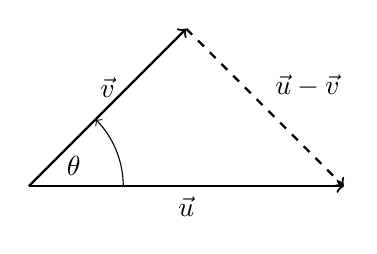
\begin{tikzpicture}[scale=2]
    \draw[thick,->] (0,0) node[anchor=south west]{$\ \ \ \theta$} -- node[anchor=north]{$\vec{u}$} (2,0);
    \draw[thick,->] (0,0) -- node[anchor=south]{$\vec{v}$} (1,1);
    \draw[thick,->, dashed] (1,1) -- node[anchor=south west]{$\vec{u} - \vec{v}$} (2,0);
    \draw[->,thin] (3/5,0) arc [start angle=0, end angle=45, radius=3/5];
\end{tikzpicture}
\end{center}
\begin{enumerate}
\item Use the Law of Cosines to show that
\[
\norm{\vec{u}-\vec{v}}^2
=\norm{\vec{u}}^2+\norm{\vec{v}}^2-2\norm{\vec{u}}\norm{\vec{v}}\cos\theta.
\]

\item  Use (a) and the previous problem to conclude the formula 
\[\vec{u}\cdot\vec{v}=\norm{\vec{u}}\norm{\vec{v}}\cos\theta.\]
\end{enumerate}}{}

\exercise{Suppose we know that $\norm{\vec{u}}=5$, $\norm{\vec{v}}=4$, and the angle between $\vec{u}$ and $\vec{v}$ is $\theta=\pi/3$. Determine the following.
\begin{enumerate}
\item $\norm{\vec{u}+\vec{v}}$.
\item $\vec{u}\cdot\vec{v}$.
\item $\norm{\frac12\vec{u}+3\vec{v}}$.
\item $\norm{\vec{u}-\vec{v}}$.
\end{enumerate}}{}

\exercise{Show that the two diagonals of a parallelogram intersect in right angles if and only if all four sides of the parallelogram have the same length.}{}

\exercise{Show that for any two vectors $\vec{u}$ and $\vec{v}$ we have
\[\abs{\vec{u}\cdot\vec{v}}\leq\norm{\vec{u}}\norm{\vec{v}}.\]
This is called the \emph{Cauchy-Schwarz inequality}.}{}

\exercise{Show that for any two vectors $\vec{u}$ and $\vec{v}$ we have
\[\norm{\vec{u}+\vec{v}}\leq\norm{\vec{u}}+\norm{\vec{v}}.\]
This is called the \emph{triangle inequality}.  Explain the name.}{}
